% !TEX root = Master.tex


To gain some insights on a hierarchical level of interest, some quick analysis is performed on different groups (nodes) of the key category cluster level in the tree (see \autoref{fig:article_hierarchy}). We start out with a broad picture on this upper level 
%in Subsection \ref{sssec:kcc_exploration} 
and eventually reach a better understanding for the the article behaviour.
\\



By viewing the sale trends separately for each key category cluster, we can observe in \autoref{fig:ts_log_sales_kcc} that, among the weekly noise, they climax similarly. Just like in the previous section, those peaks come about primarily during the big promotions weeks. To put it into perspective, we can see logarithmic sale behaviour in \autoref{fig:boxplot_log_sales_kcc}, were patterns are quite similar although they differ strongly in volume. 
\\

 \begin{figure}[H]
\centering
\begin{subfigure}{.45\textwidth}
  \centering
  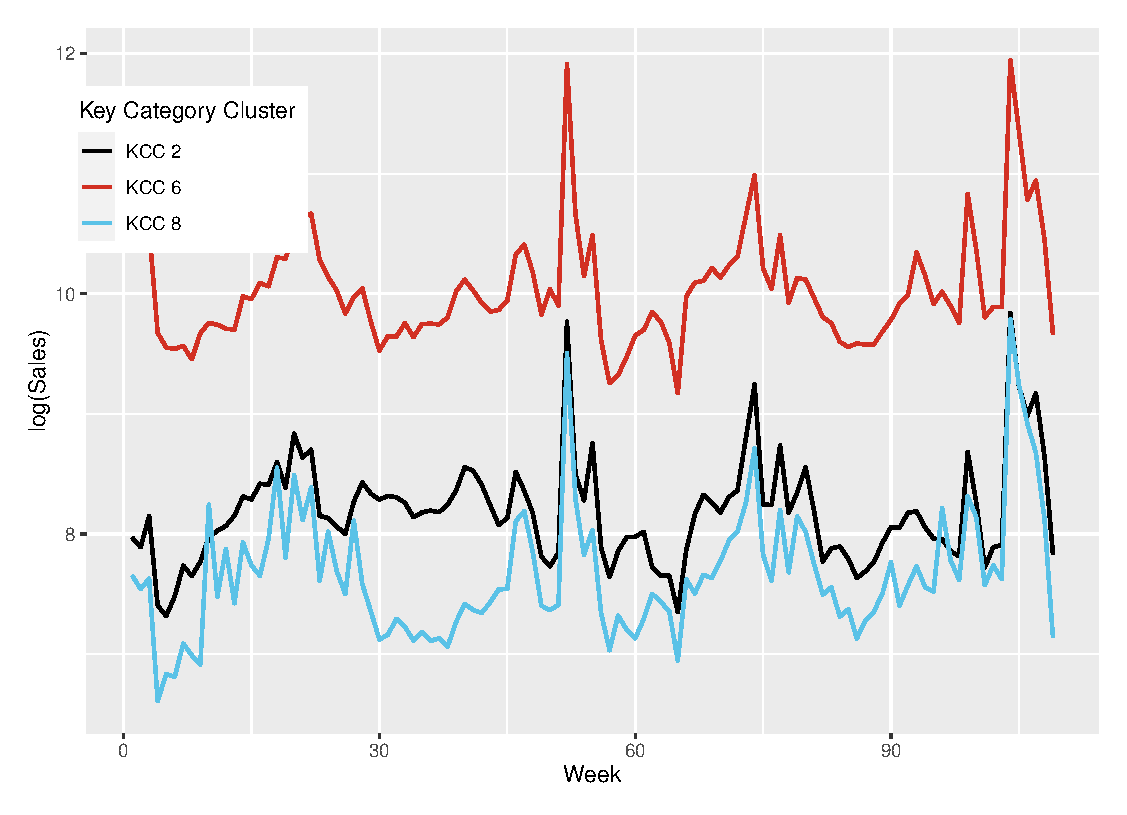
\includegraphics[width=\linewidth]{figures/ts_log_sales_kcc.eps}
  \caption{Time series of log(Sales) per KCC}
  \label{fig:ts_log_sales_kcc}
\end{subfigure}
\begin{subfigure}{.45\textwidth}
  \centering
  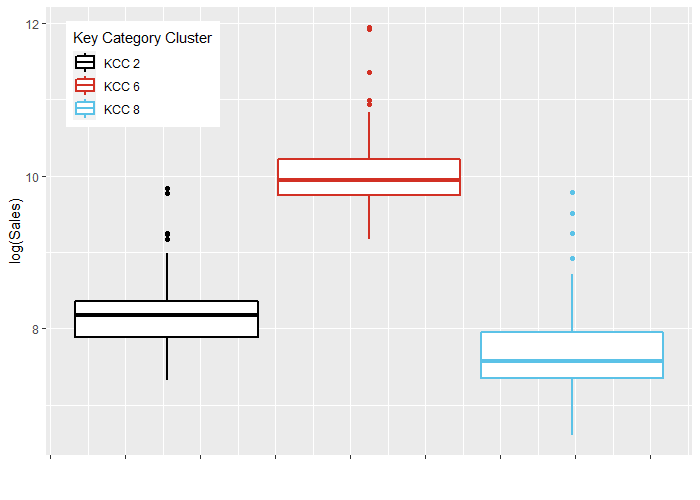
\includegraphics[width=\linewidth]{figures/boxplot_log_sales_kcc.png}
  \caption{Boxplots of log(Sales) per KCC}
  \label{fig:boxplot_log_sales_kcc}
\end{subfigure}
\caption{Time series and boxplot showing logarithmized sales of the key category clusters}
\label{fig:kcc_ts_and_boxplot}
\end{figure} 




\begin{figure}[H]
\centering
  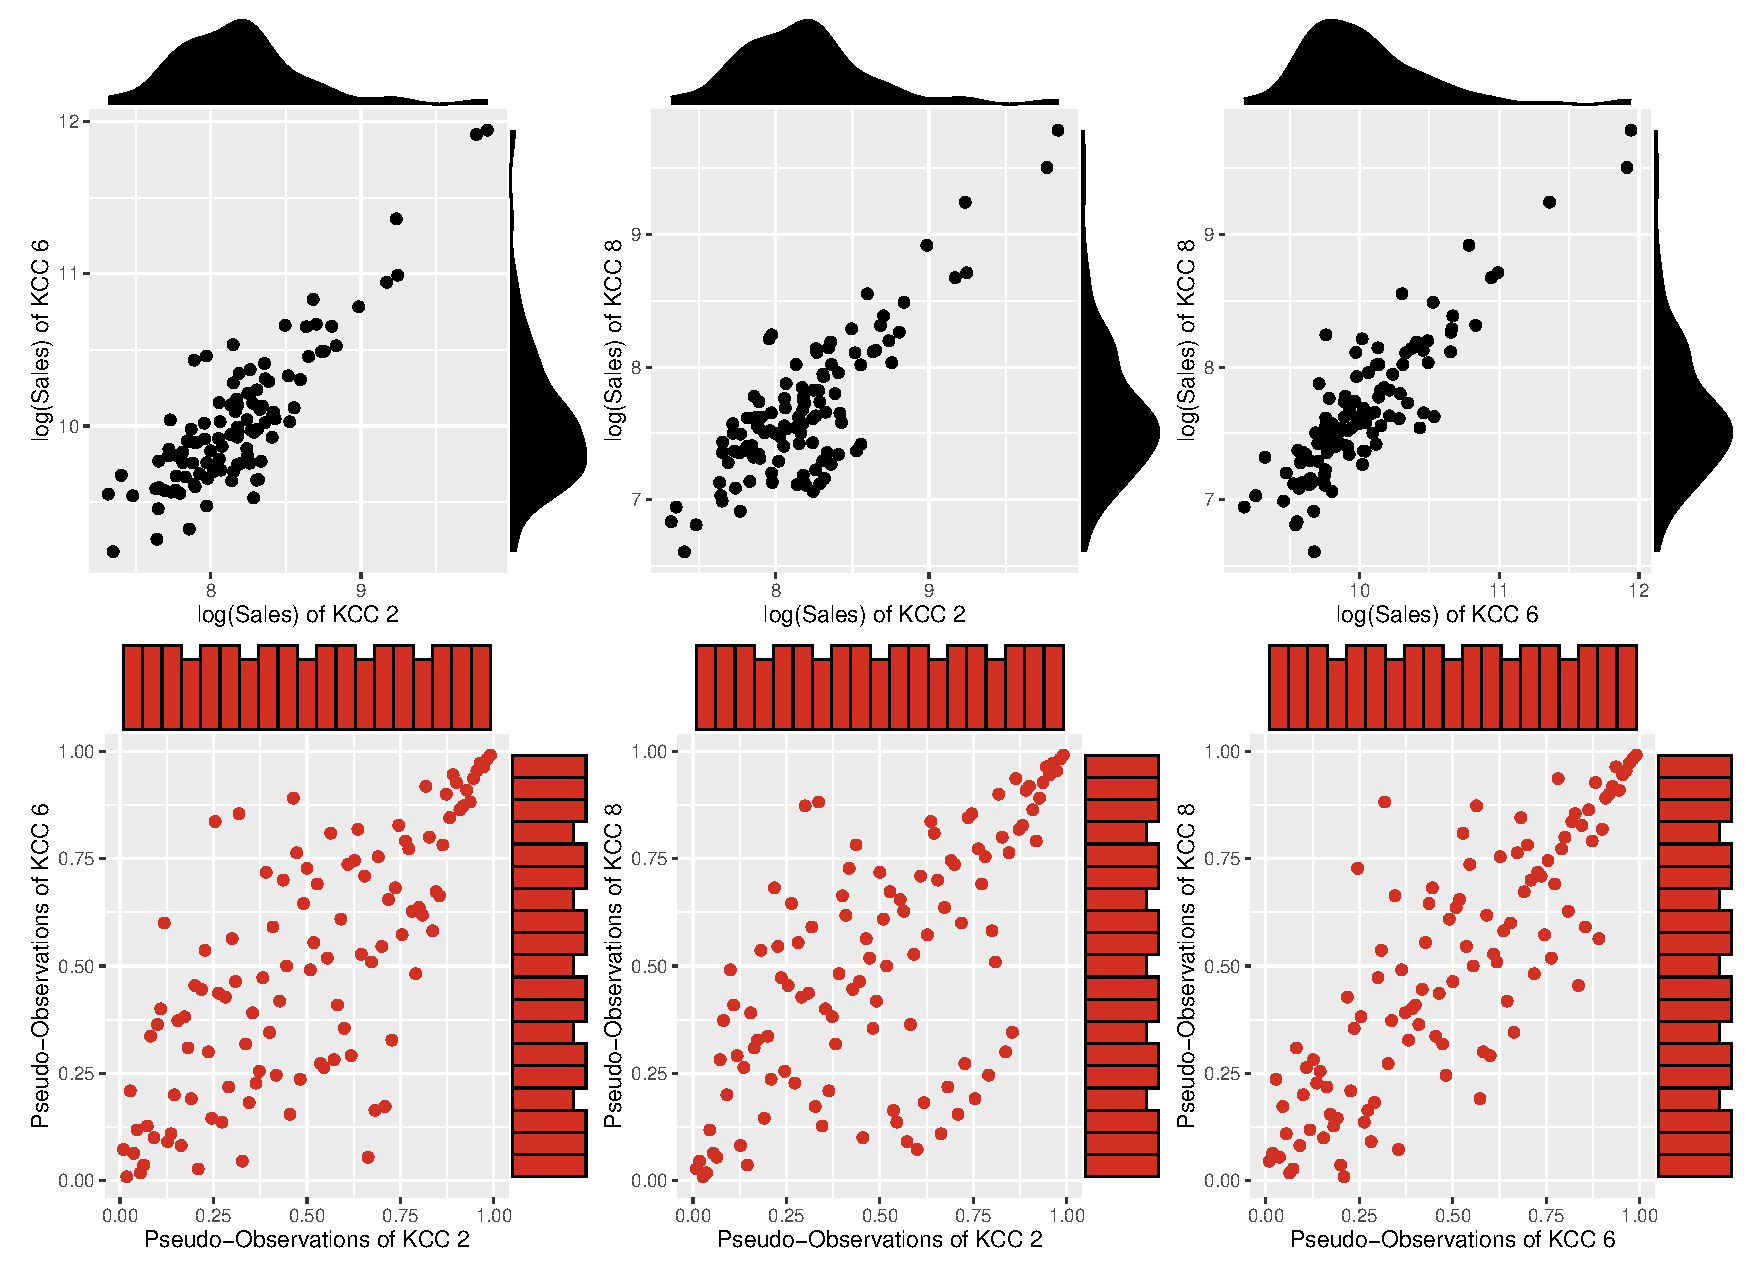
\includegraphics[width=0.95\linewidth]{figures/kcc_pair_scatterplots.eps}
  \caption{Pairwise scatterplots of sales on \ac{KCC} level. First row: Logarithmic sales with marginal densities, Second row: Pseudo sales observation with marginal histograms}
  \label{fig:kcc_pair_scatterplots}
\end{figure}


All the more interesting are the joint distributions of our \acp{KCC}. \autoref{fig:kcc_pair_scatterplots} shows scatterplots of \ac{KCC} pairs. In the first row we can see some isolated points on the upper tails representing outliers. We took the logarithmized sales to spot differences that would be otherwise hard to see. The outliers produced by the promotions still remain outliers in the log-scale. Also, by checking the densities for the margins, pertinent marginal distributions are hardly determined but not to be ruled out.\\
The second row displays the pairs of the according \textit{pseudo observations}. Pseudo observations are calculated by taking the data ranks and dividing them by "1 + number of observations", which makes them robust against outliers and restricts the value range to $(0, 1)$. Here we are faced with a strange behaviour of the histograms. They practically look uniformly distributed, however there are seemingly regular step patterns in the pseudo data. This might be traced back to the fact that we are dealing in reality with discrete data of not necessarily unique occurrence.\\

For the above reasons, on \ac{KCC} level we will attempt modelling parametric distributions to the margins (see Chapter \ref{sec:modelling}). 
%The reason being for the latter is that our primary objective is to capture a dependence structure, whereas the margins per se are of secondary interest. 
In addition, looking at both rows of \autoref{fig:kcc_pair_scatterplots}, we suspect tail dependence and there is an obvious strong positive correlation among all three pairs, which is confirmed by viewing \autoref{fig:corplot_kcc} displaying various correlation metrics.
 \\


\begin{figure}[H]
\centering
  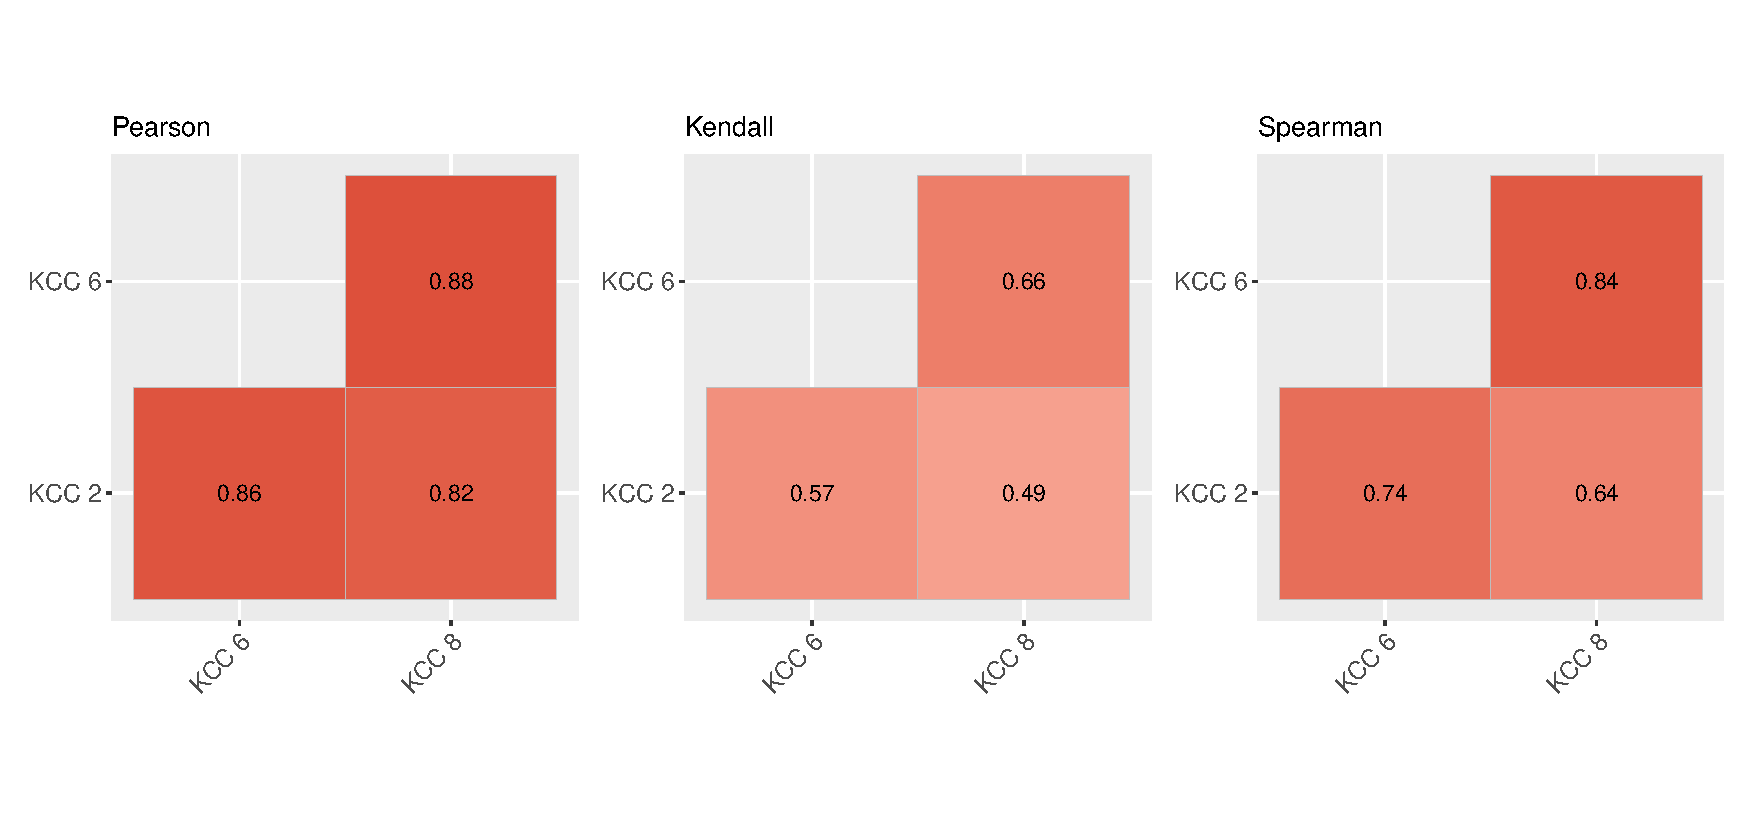
\includegraphics[width=0.95\linewidth]{figures/corplot_kcc.eps}
  \caption{Correlation plots of the three \ac{KCC} log-sales with different correlation coefficients. Left: Pearson's rho, Middle: Kendall's tau, Right: Spearman's rho}
  \label{fig:corplot_kcc}
\end{figure}




One side note on the promotion intensities of Black Friday and Friends \& Family (see \autoref{tab:transactional_data}) is that on higher levels such as key category cluster, as we aggregate our data, promotion intensities become binary values indicating whether the respective promotion took place in those respective weeks. Also note that Black Friday and Friends \& Family weeks do not overlap. The boxplots of the two promotion types depicted in \autoref{fig:bf_kcc_boxplot} and \autoref{fig:ff_kcc_boxplot} point out how they affect the sales. Though, one shall keep in mind that, out of 109 weeks, only the minority include promo activation. Precisely, Black Friday is activated over 6 weeks out of 109 and Friends \& Family is activated over 13 weeks\footnote{And of course not in a row, as can be clearly observed in \autoref{fig:total_sold_articles_ts}.} (see Tables \ref{tab:black_friday} and \ref{tab:friends_and_family}). In \autoref{fig:ff_kcc_boxplot}, one shall also be aware of large outliers being present during no Friends \& Family weeks, which is fairly aligned with what we figured out in the previous subsection (i.e. many sale occurrences do not have any promotion).
\\


\begin{figure}[H]
\centering
  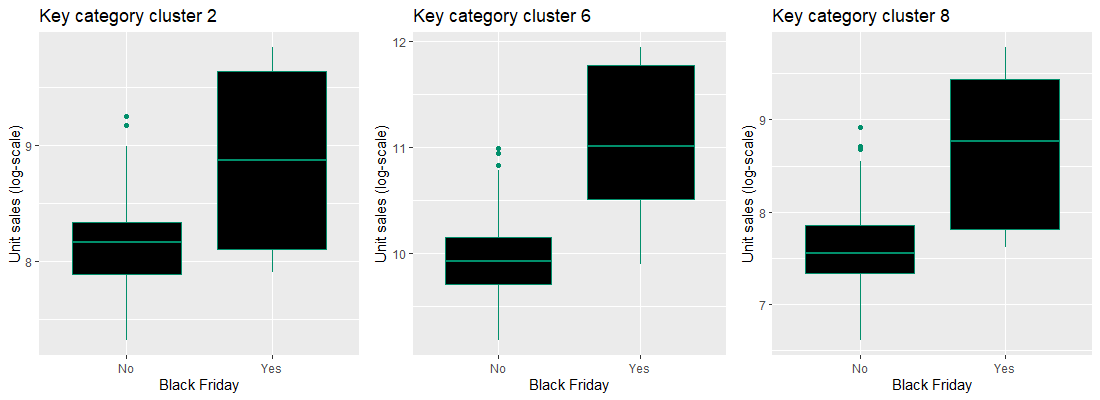
\includegraphics[width=0.95\linewidth]{figures/bf_kcc_boxplot.png}
  \caption{Boxplots showing log-sales of KCCs against presence of Black Friday}
  \label{fig:bf_kcc_boxplot}
\end{figure}


\begin{figure}[H]
\centering
  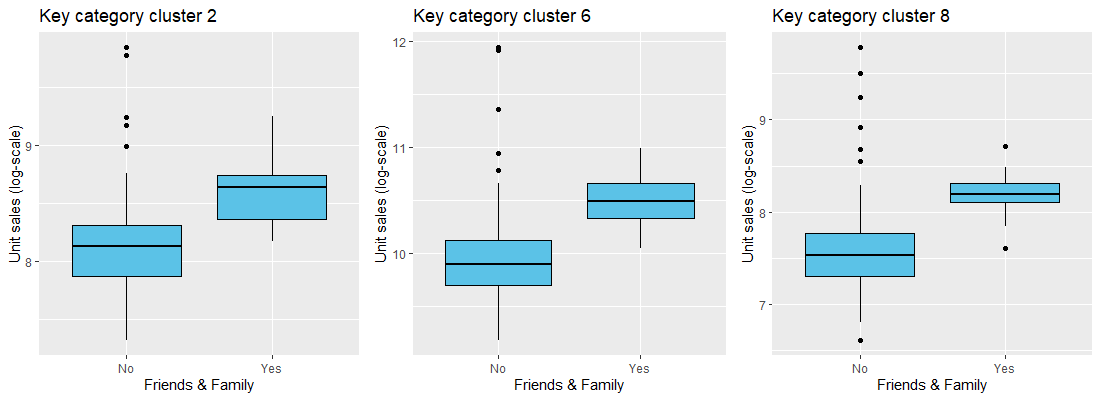
\includegraphics[width=0.95\linewidth]{figures/ff_kcc_boxplot.png}
  \caption{Boxplots showing log-sales of KCCs against presence of Friends \& Family}
  \label{fig:ff_kcc_boxplot}
\end{figure}


The scatterplots in \autoref{fig:total_markdown_against_kcc} clearly reveal the strong positive relationship between the log-sales and the \ac{KCC}s' respective total markdown percentages.
\\
Regarding the season type (SS vs FW), visual exploration is not sufficient to conclude existence of effects on the unit sales. The effect of season type as well as other features on the unit sales shall be discussed in Chapter \ref{sec:modelling}.
\\




\begin{figure}[H]
\centering
  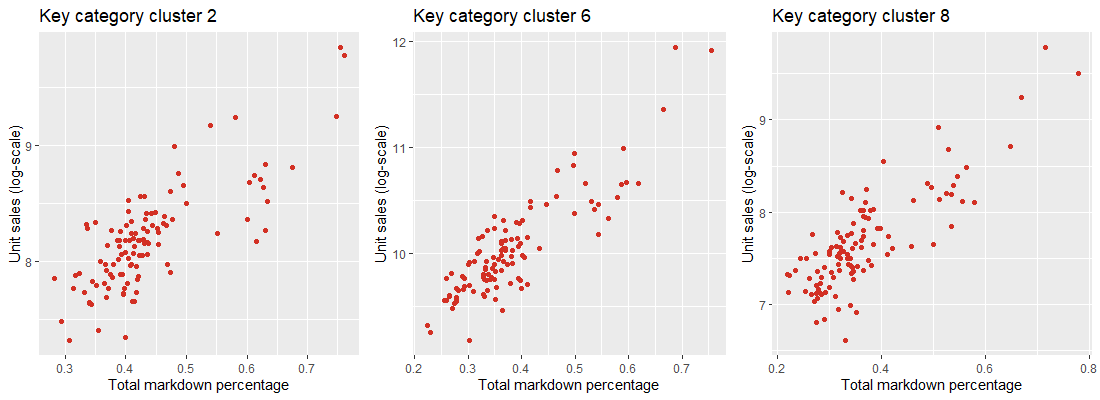
\includegraphics[width=0.95\linewidth]{figures/total_markdown_against_kcc.png}
  \caption{Scatterplots of \ac{KCC} log-sales against total markdown percentage}
  \label{fig:total_markdown_against_kcc}
\end{figure}






\begin{figure}[H]
\centering
  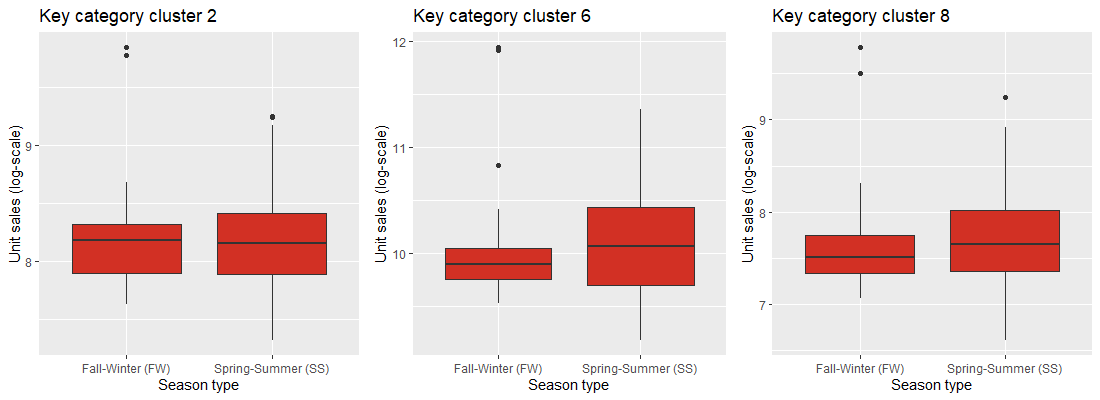
\includegraphics[width=0.95\linewidth]{figures/season_type_against_kcc.png}
  \caption{Boxplots of \ac{KCC} log-sales against the two season types}
  \label{fig:season_type_against_kcc}
\end{figure}





